\newpage
\section{Chapitre 4 : Analyse et conception du système}

Ce chapitre présente l'analyse fonctionnelle du système CYBEL ainsi que les
choix de conception retenus pour répondre au cahier des charges défini au
chapitre précédent. Il détaille successivement les acteurs et les besoins
identifiés, l'architecture générale et logicielle de la plateforme, les
diagrammes de conception (composants, cas d'utilisation, séquence) et le
modèle des flux de communication entre les différents sous-systèmes.

\subsection{Analyse fonctionnelle}

Après l'étude du besoin et l'analyse des solutions existantes, il est
nécessaire de définir précisément le fonctionnement du système à concevoir.
Cette phase d'analyse fonctionnelle permet d'identifier les acteurs
intervenant dans le système, les services qui leur sont proposés ainsi que
les interactions nécessaires à la réalisation des différentes
fonctionnalités.

Le projet CYBEL vise à fournir une plateforme de supervision, de commande
et d'interaction destinée au robot de service CIOT TY1251D-03195, déployé
au sein du FabLab de HESTIM. Cette plateforme doit permettre aux opérateurs
de piloter le robot, de suivre son état en temps réel et de gérer les
interactions avec les visiteurs, tout en assurant une communication fiable
avec les différents composants matériels et logiciels du système.

L'analyse fonctionnelle constitue ainsi une étape essentielle avant la
conception détaillée de l'architecture, puisqu'elle permet de traduire les
besoins exprimés dans le cahier des charges en fonctionnalités concrètes.

\subsubsection{Identification des acteurs}

L'étude des besoins a permis d'identifier trois acteurs principaux
intervenant dans le fonctionnement du système CYBEL.

\paragraph{L'opérateur.}
L'opérateur représente l'utilisateur chargé de l'administration et de la
supervision du robot. Il dispose d'une interface lui permettant de
consulter l'état du robot, de visualiser sa position sur la carte,
d'accéder aux informations de télémétrie, de lancer des scénarios de
navigation, de téléopérer le robot, de déclencher des annonces vocales et
de gérer les paramètres du système. Son rôle est central puisque c'est lui
qui assure le contrôle opérationnel du robot au sein du FabLab.

\paragraph{Le visiteur.}
Le visiteur interagit avec le robot à travers l'interface embarquée sur la
tablette Android. Cette interface lui permet notamment de découvrir les
différents espaces du FabLab, de sélectionner des points d'intérêt, de
consulter des informations de présentation et d'interagir avec le robot
lors des démonstrations. Le visiteur n'a pas accès aux fonctionnalités
d'administration ou de contrôle du système.

\paragraph{Le système CYBEL.}
Le système CYBEL constitue un acteur autonome chargé de coordonner les
différents composants logiciels. Il assure notamment la collecte des
données du robot, la diffusion de la télémétrie, la gestion des
communications, la reconnexion automatique en cas de perte de liaison, la
synchronisation des données entre les interfaces, ainsi que le
déclenchement des services associés à la navigation et à l'interaction.

\subsubsection{Besoins fonctionnels}

À partir de l'analyse du besoin, plusieurs fonctionnalités principales ont
été identifiées.

\paragraph{Supervision du robot.}
Le système doit permettre la consultation en temps réel du niveau de
batterie, de la position du robot, de son état de navigation, des données
LiDAR, des visiteurs détectés et des messages de diagnostic.

\paragraph{Navigation autonome.}
Le système doit permettre l'envoi du robot vers un point prédéfini, la
navigation vers une position sélectionnée sur la carte, l'annulation d'une
mission en cours, ainsi que le suivi de l'avancement de la navigation.

\paragraph{Téléopération.}
L'opérateur doit pouvoir contrôler manuellement les déplacements du robot
à travers une interface de commande ou un clavier virtuel.

\paragraph{Interaction Homme-Robot.}
Le système doit permettre le déclenchement d'annonces vocales, la
diffusion de messages d'accueil, l'utilisation de commandes vocales
opérateur, ainsi que l'affichage d'informations destinées aux visiteurs.

\paragraph{Configuration du système.}
L'opérateur doit pouvoir modifier certains paramètres de fonctionnement
tels que les vitesses de déplacement, les paramètres de navigation et les
réglages de communication.

\paragraph{Mode simulation.}
Le système doit être capable de fonctionner sans robot physique grâce à un
mode simulé permettant le développement et les tests des fonctionnalités.

\subsubsection{Besoins non fonctionnels}

Outre les fonctionnalités attendues, plusieurs contraintes de qualité ont
été retenues.

\paragraph{Performance.}
La plateforme doit assurer une mise à jour rapide des informations afin de
garantir une supervision efficace du robot.

\paragraph{Fiabilité.}
Le système doit maintenir la continuité des communications et assurer une
reconnexion automatique après une interruption réseau.

\paragraph{Maintenabilité.}
L'architecture doit favoriser l'évolution et la réutilisation du code
grâce à une séparation claire des responsabilités.

\paragraph{Sécurité.}
Les commandes critiques doivent pouvoir être annulées rapidement afin
d'éviter tout comportement indésirable du robot.

\paragraph{Ergonomie.}
Les interfaces doivent être simples d'utilisation et adaptées aussi bien
aux opérateurs qu'aux visiteurs.

\subsection{Architecture générale de CYBEL}

Afin de répondre aux besoins identifiés, une architecture modulaire a été
retenue. Celle-ci repose sur plusieurs composants indépendants
communiquant entre eux à travers des interfaces clairement définies.
L'objectif principal de cette architecture est de découpler les interfaces
utilisateur du système robotique afin de faciliter les tests, la
maintenance et l'évolution de la plateforme.

\begin{figure}[h!]
    \centering
    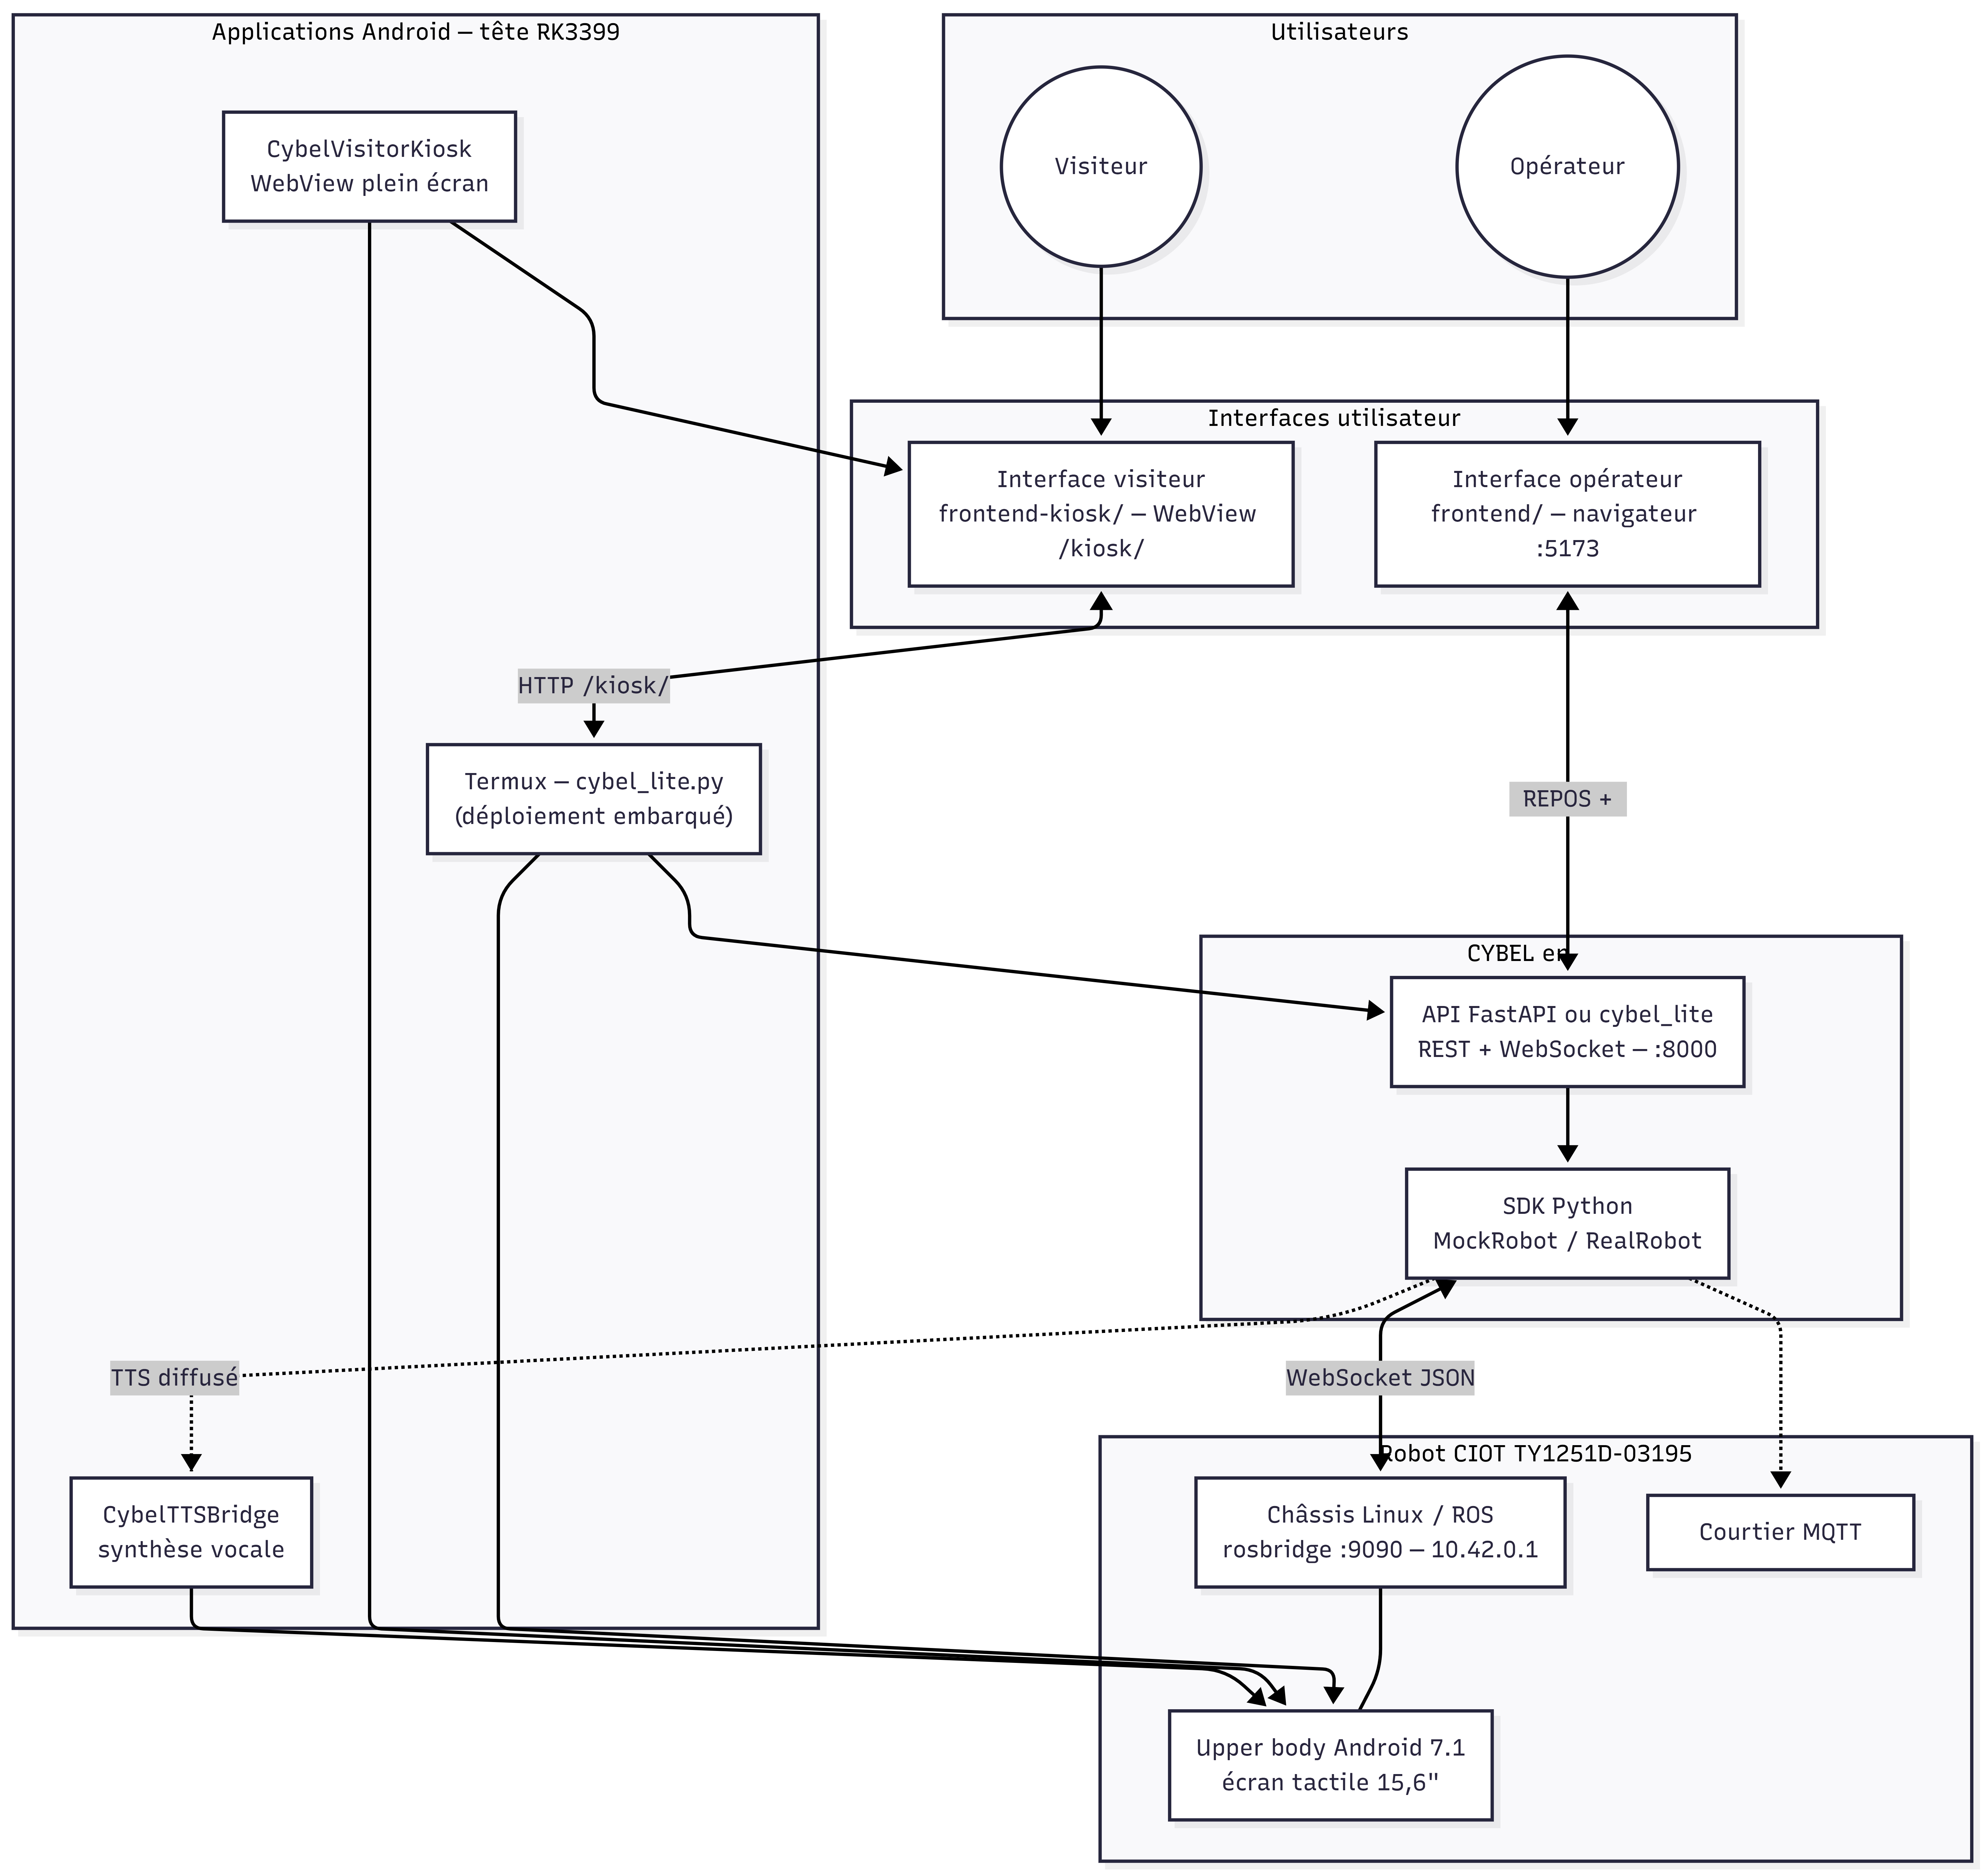
\includegraphics[width=0.9\textwidth]{diagramme/architecture_generale.png}
    \caption{Architecture générale du système CYBEL}
    \label{fig:archi_generale_cybel}
\end{figure}

Comme illustré en figure~\ref{fig:archi_generale_cybel}, l'architecture
globale du système s'articule autour de quatre ensembles principaux : le
robot CIOT TY1251D-03195, le backend CYBEL, les interfaces utilisateur et
les applications Android embarquées. Chaque composant joue un rôle
spécifique dans le fonctionnement global de la plateforme.

\subsection{Architecture logicielle}

L'architecture logicielle retenue suit une approche en couches permettant
de séparer les responsabilités fonctionnelles et techniques du système.
Elle est organisée autour de trois couches principales.

\subsubsection*{Couche d'accès au robot (SDK)}

Cette couche constitue l'abstraction du robot. Elle est responsable de la
communication avec ROSBridge, de la gestion du protocole reconstruit, de
l'accès aux données de télémétrie et de l'exécution des commandes. Deux
implémentations sont proposées : une implémentation réelle et une
implémentation simulée. Cette approche permet de développer et de tester
la plateforme sans dépendre de la disponibilité permanente du robot.

\subsubsection*{Couche API}

Cette couche repose sur FastAPI et constitue le point d'entrée principal
du système. Elle expose des services REST, des services WebSocket ainsi
que les mécanismes de gestion des événements. Elle joue également le rôle
d'intermédiaire entre les interfaces utilisateur et le SDK.

\subsubsection*{Couche présentation}

Cette couche regroupe l'interface opérateur, l'interface visiteur et les
applications Android complémentaires. Elle permet l'interaction entre les
utilisateurs et le système.

\begin{center}
    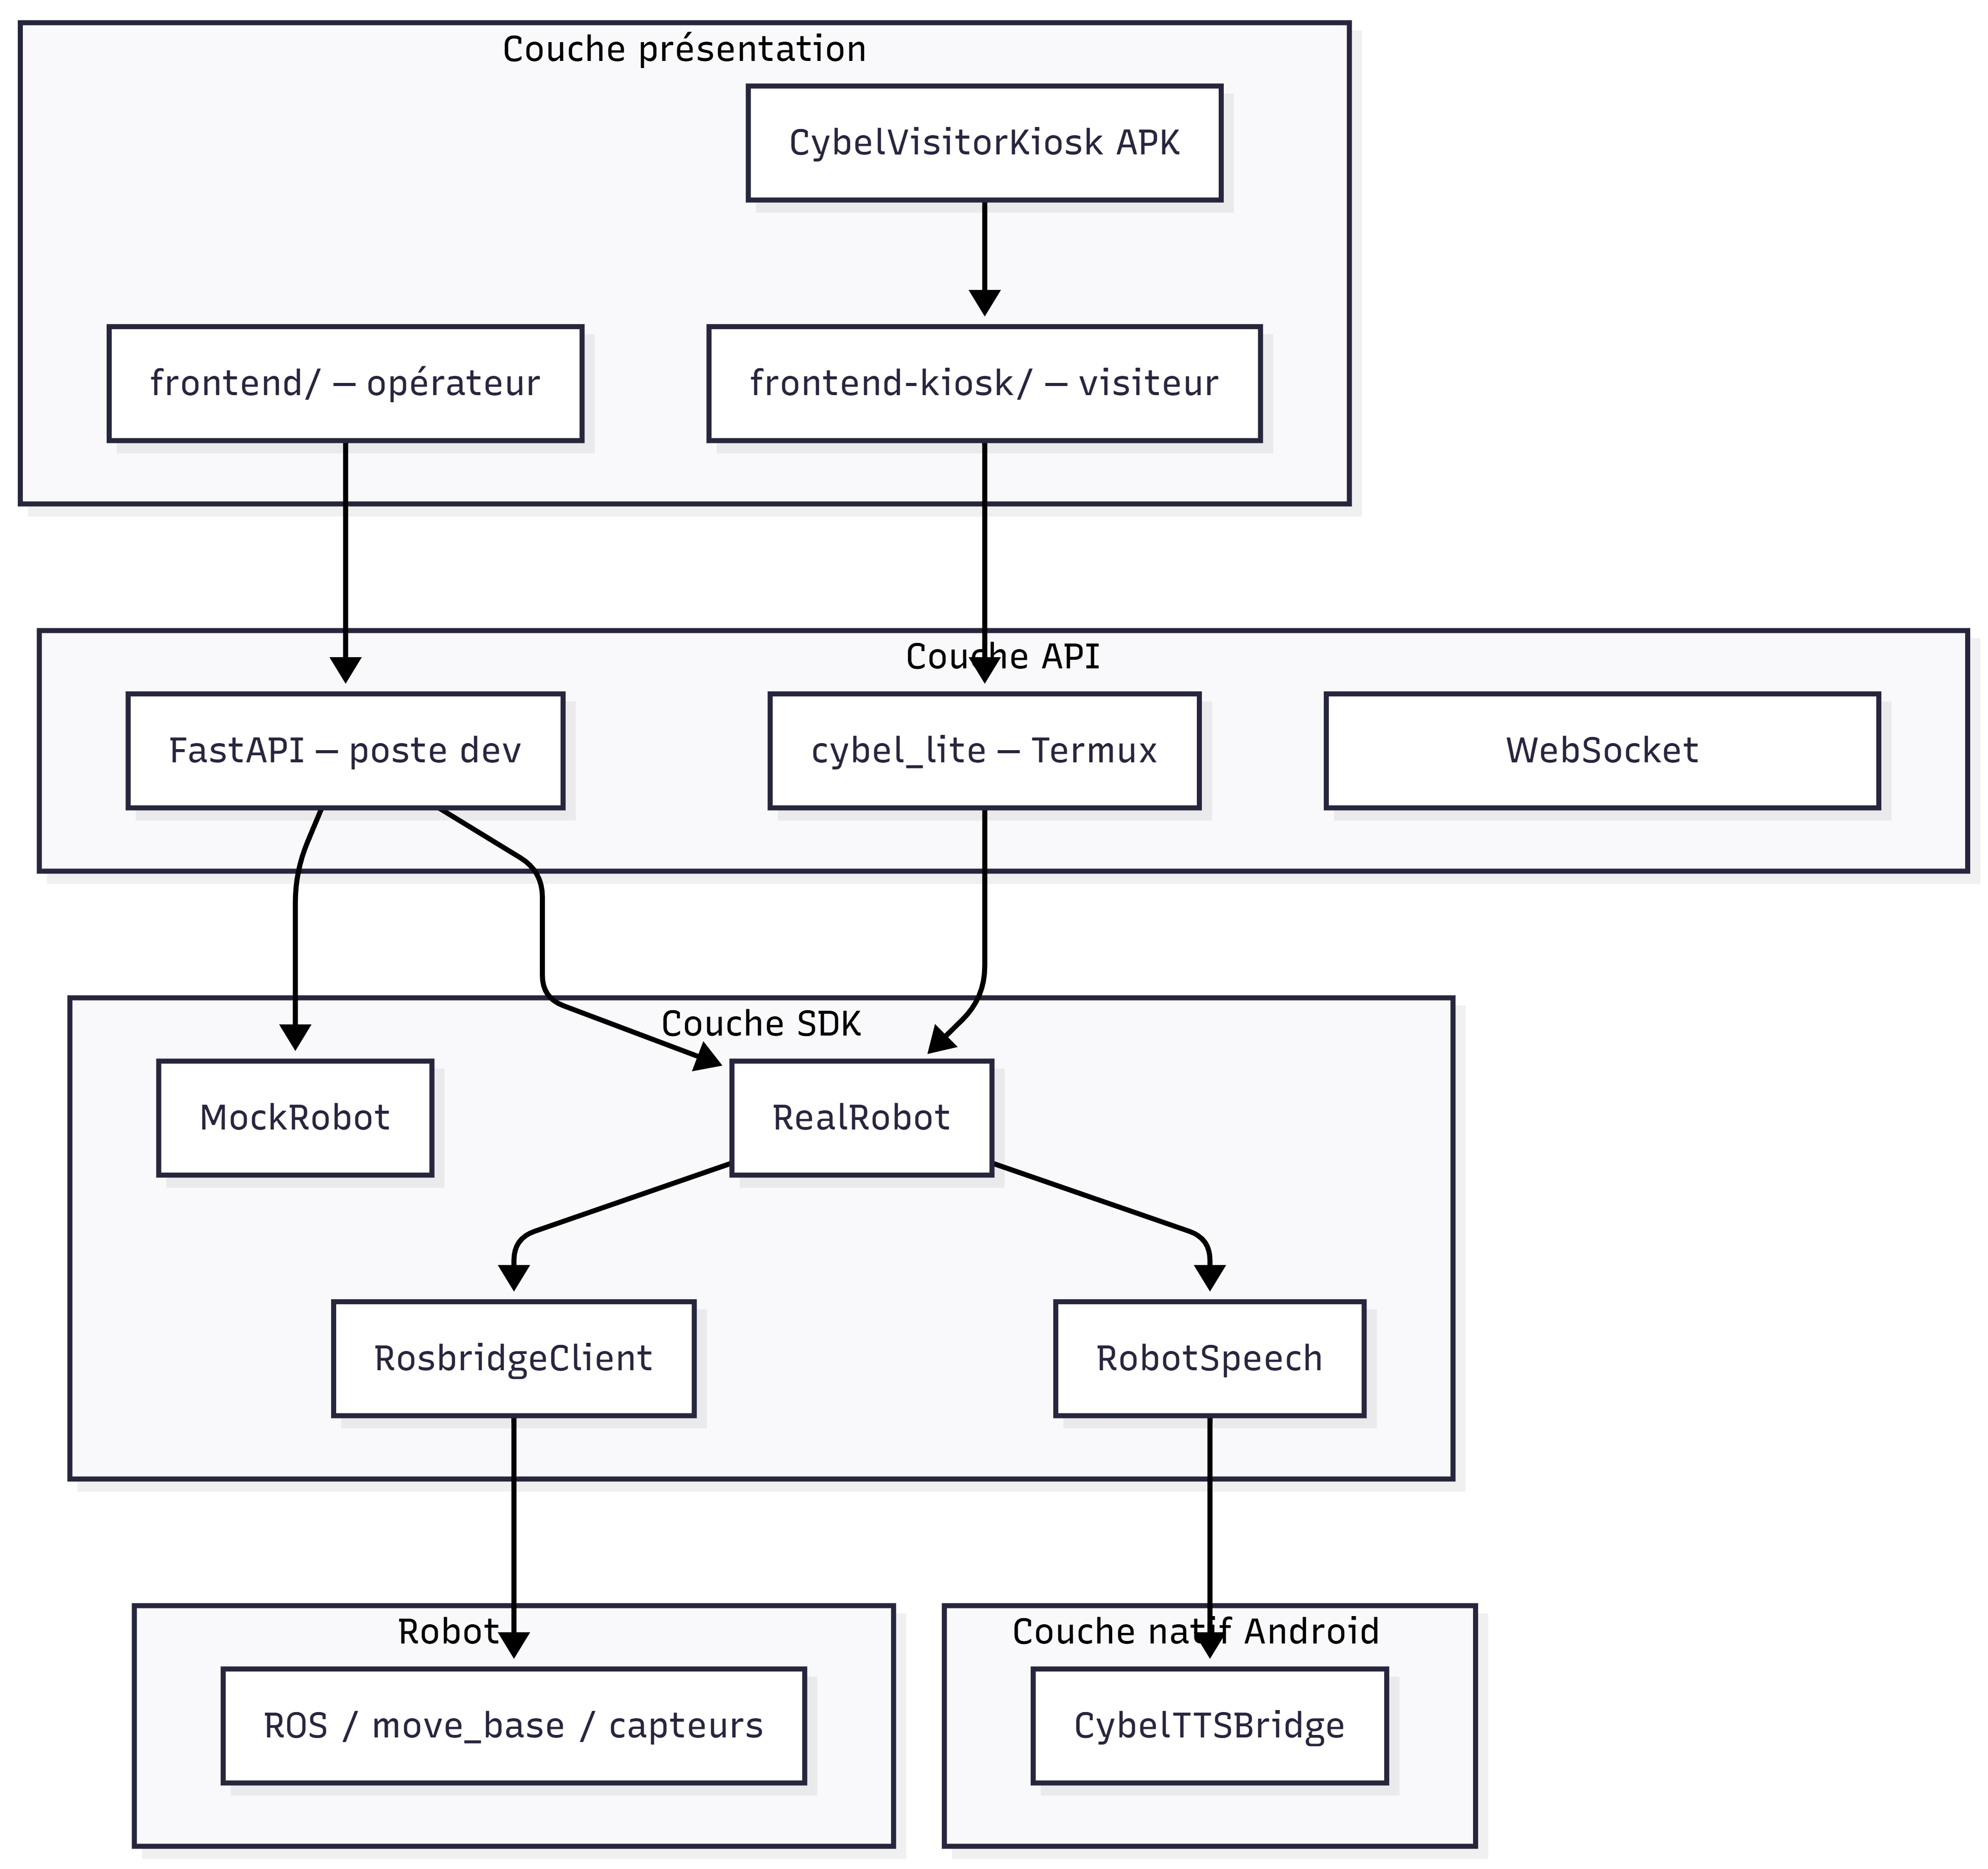
\includegraphics[width=0.8\textwidth]{diagramme/Architecture en couches-2026-06-20-163125.png}
    \captionof{figure}{Architecture en couches}
\end{center}

\subsection{Diagramme des composants}

Le diagramme des composants (figure~\ref{fig:diag_composants}) met en
évidence l'organisation des différents modules logiciels du système ainsi
que leurs dépendances. Il montre notamment les interfaces opérateur et
visiteur, le backend FastAPI, le SDK robot, ROSBridge, le système Android
embarqué ainsi que les modules TTS. Cette représentation permet de
visualiser clairement la répartition des responsabilités entre les
différents composants.

\begin{figure}[h!]
    \centering
    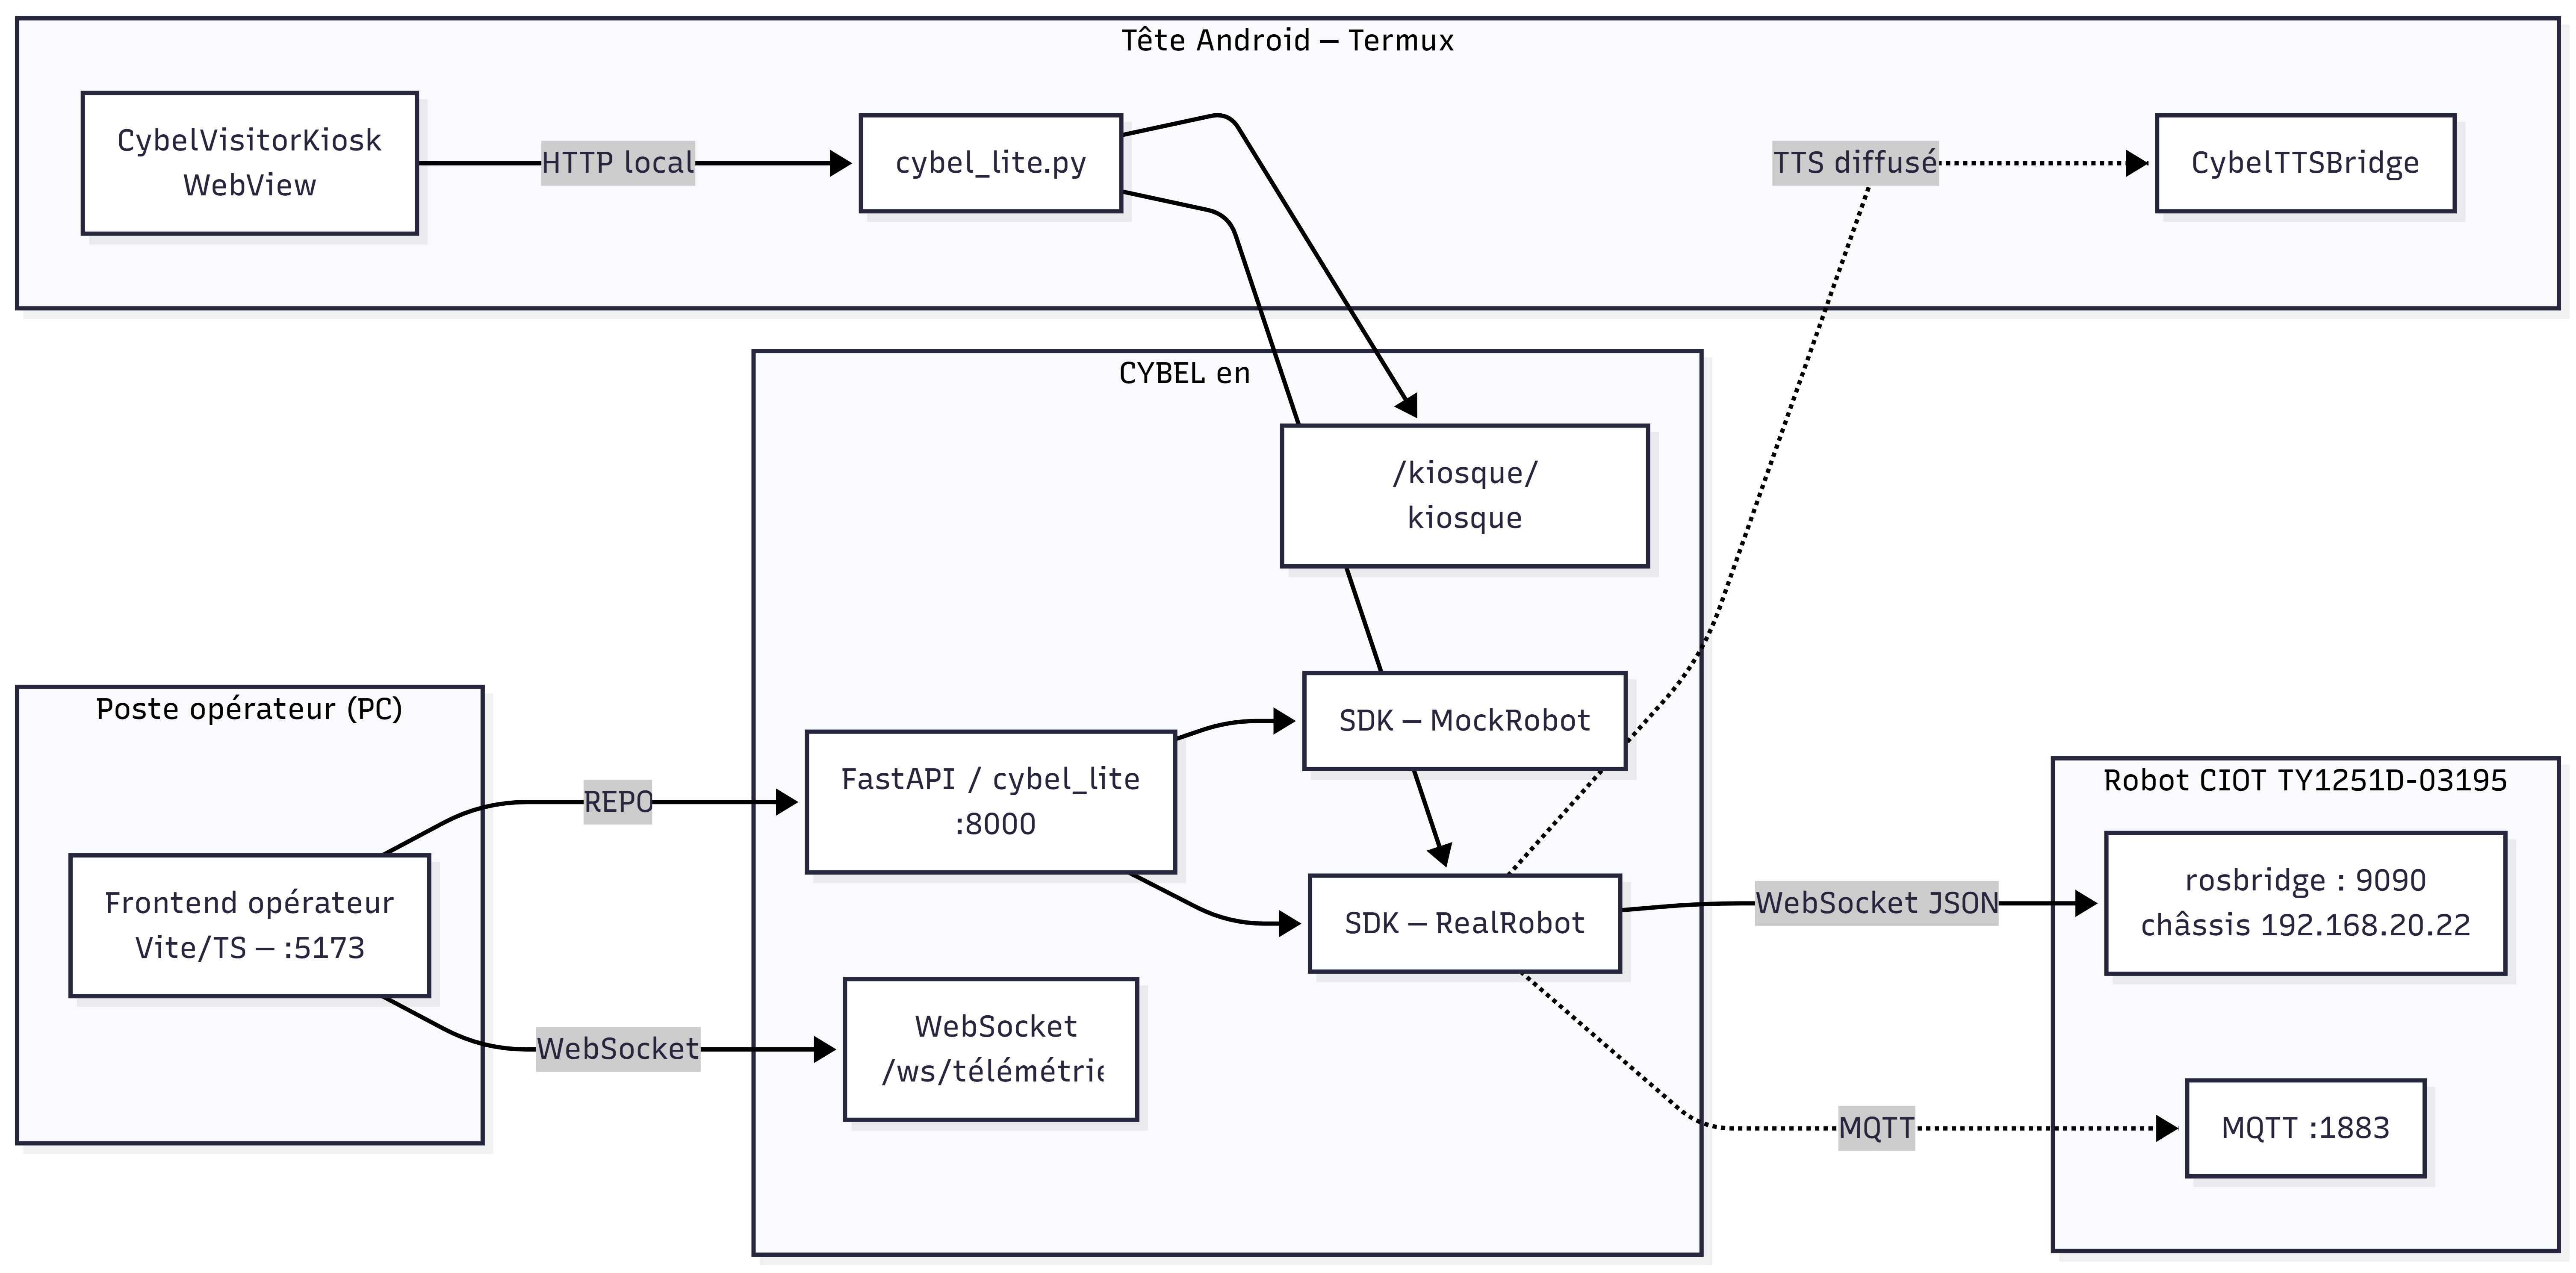
\includegraphics[width=0.85\textwidth]{diagramme/diagramme_composant.png}
    \caption{Diagramme de composants du système CYBEL}
    \label{fig:diag_composants}
\end{figure}

\subsection{Diagrammes de cas d'utilisation}

Les diagrammes de cas d'utilisation (figure~\ref{fig:diag_cas_usage})
permettent de représenter les interactions entre les acteurs identifiés et
les fonctionnalités proposées par le système. Ils mettent en évidence les
actions réalisées par l'opérateur, les interactions du visiteur, ainsi que
les traitements automatiques assurés par CYBEL.

\begin{figure}[h!]
    \centering
    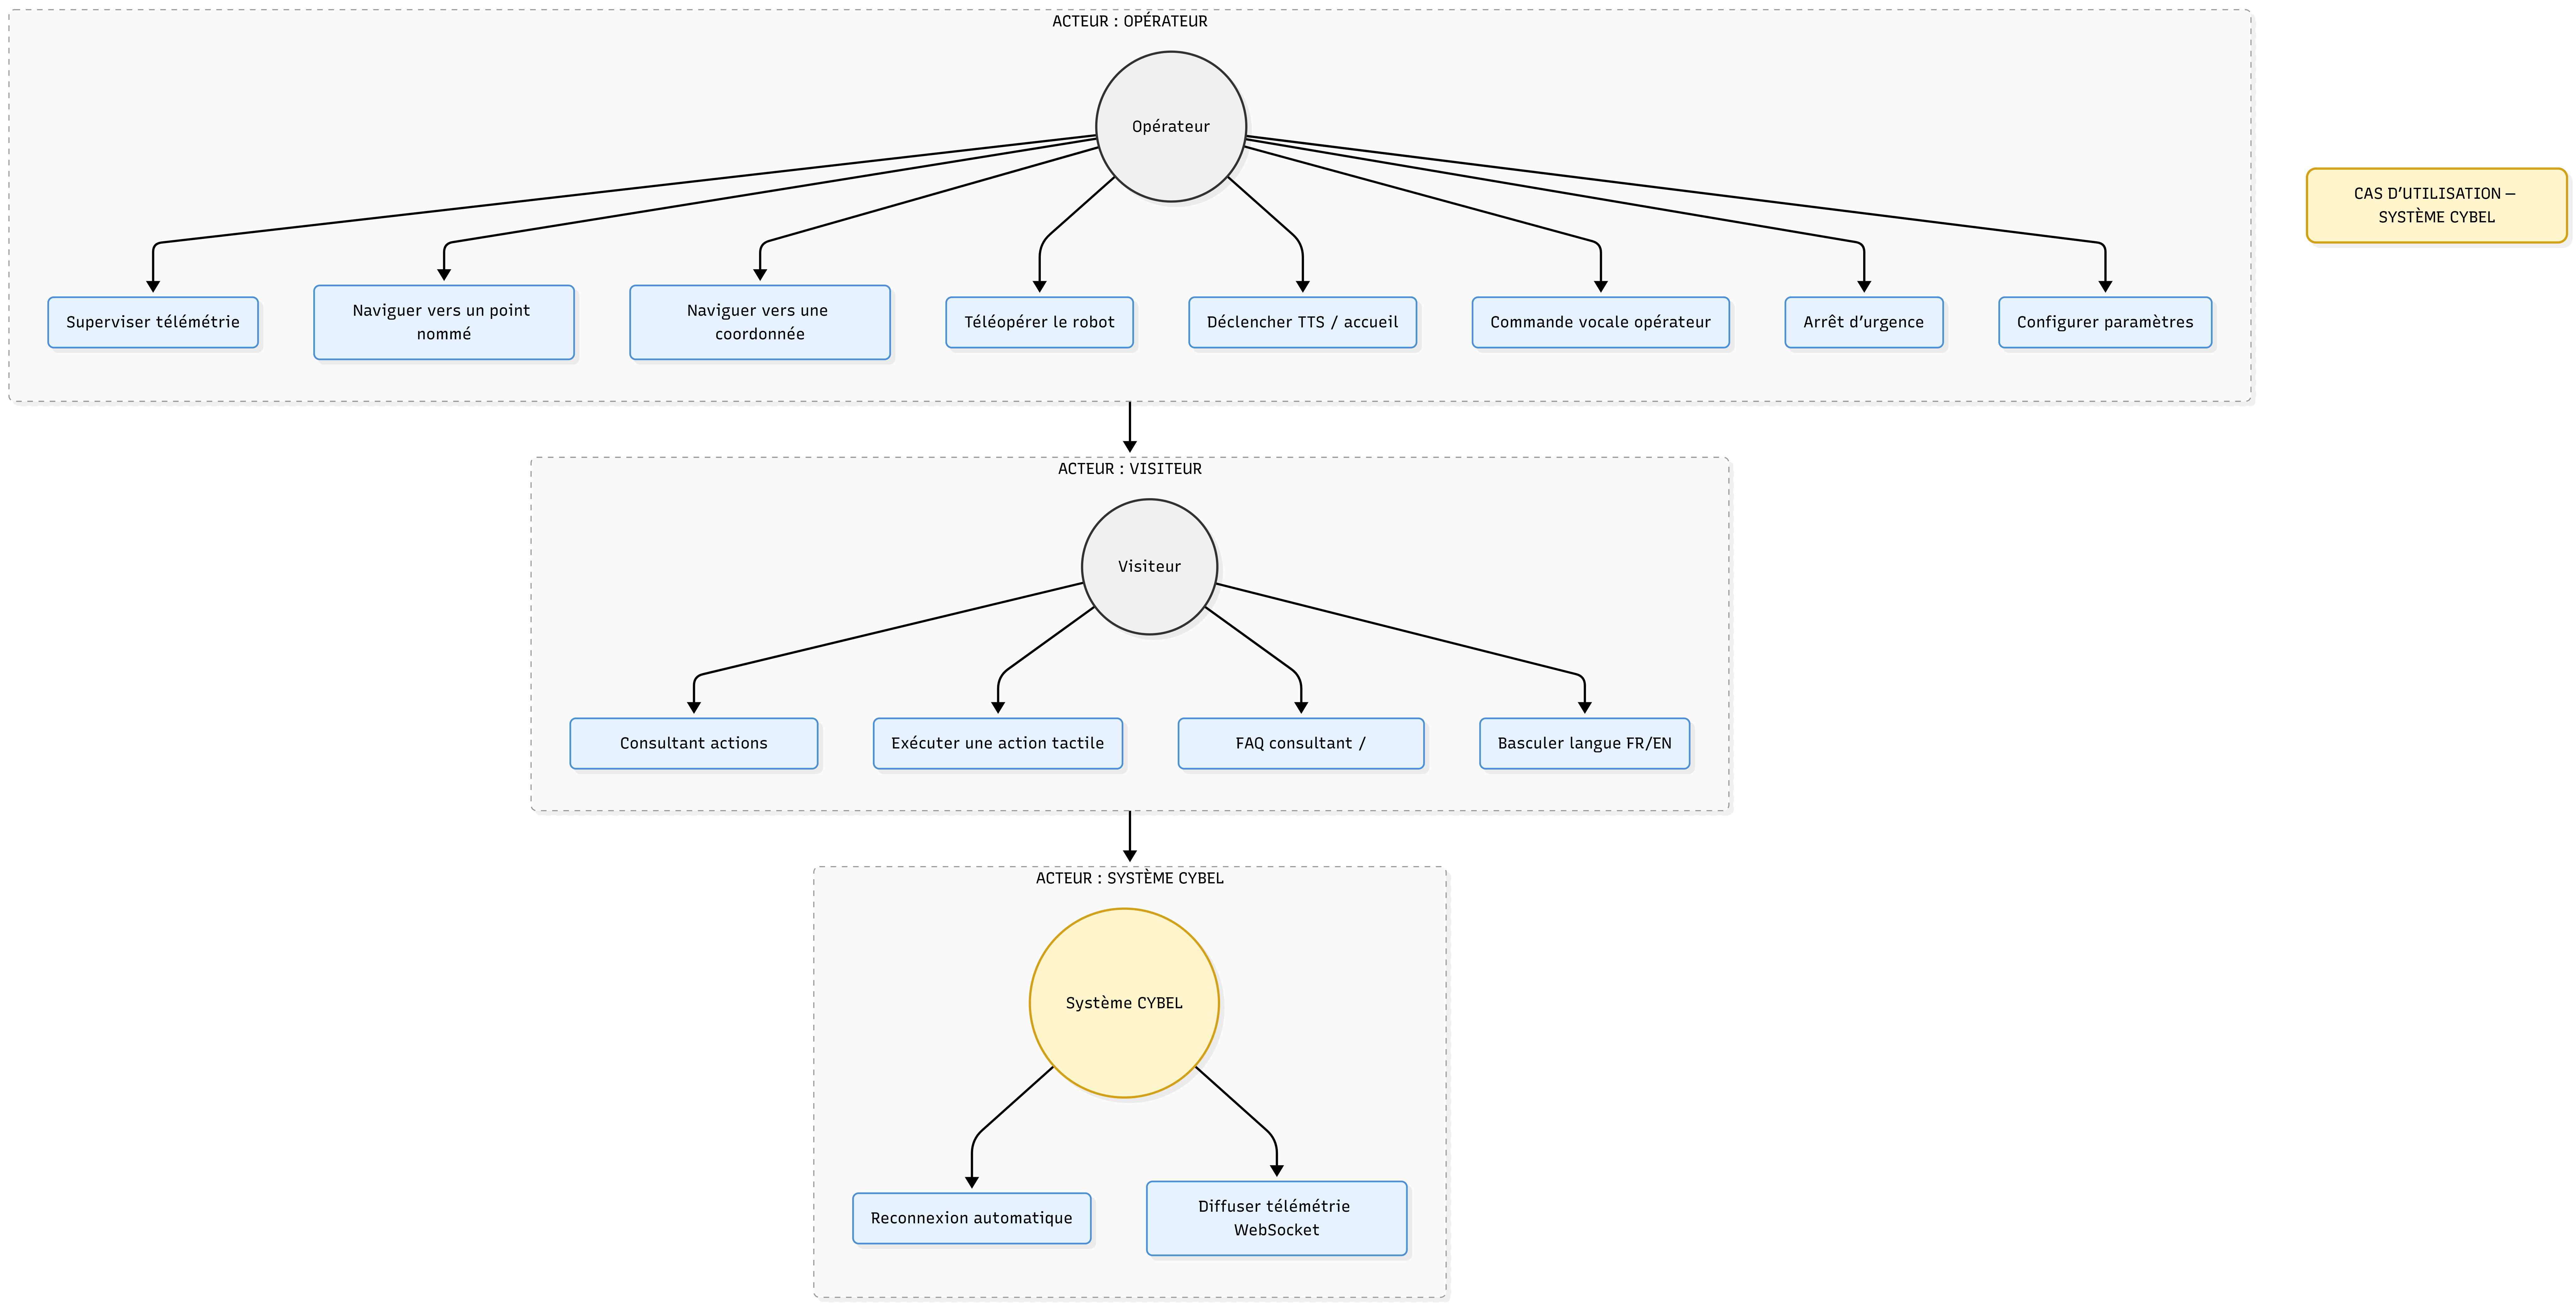
\includegraphics[width=0.9\textwidth]{diagramme/diagramme_cas_usage.png}
    \caption{Diagramme de cas d'utilisation du système CYBEL}
    \label{fig:diag_cas_usage}
\end{figure}

\subsection{Diagrammes de séquence}

Les diagrammes de séquence (figure~\ref{fig:diag_sequence}) permettent de
décrire l'enchaînement des échanges entre les différents composants du
système lors de l'exécution d'une fonctionnalité. Parmi les scénarios
étudiés figurent la navigation vers un point sélectionné, l'envoi d'une
commande de déplacement, le déclenchement d'une annonce vocale, ainsi que
la diffusion de la télémétrie vers l'interface opérateur. Ces diagrammes
facilitent la compréhension des mécanismes internes mis en \oe uvre lors
des communications entre le robot, le backend et les interfaces
utilisateur.

\begin{figure}[h!]
    \centering
    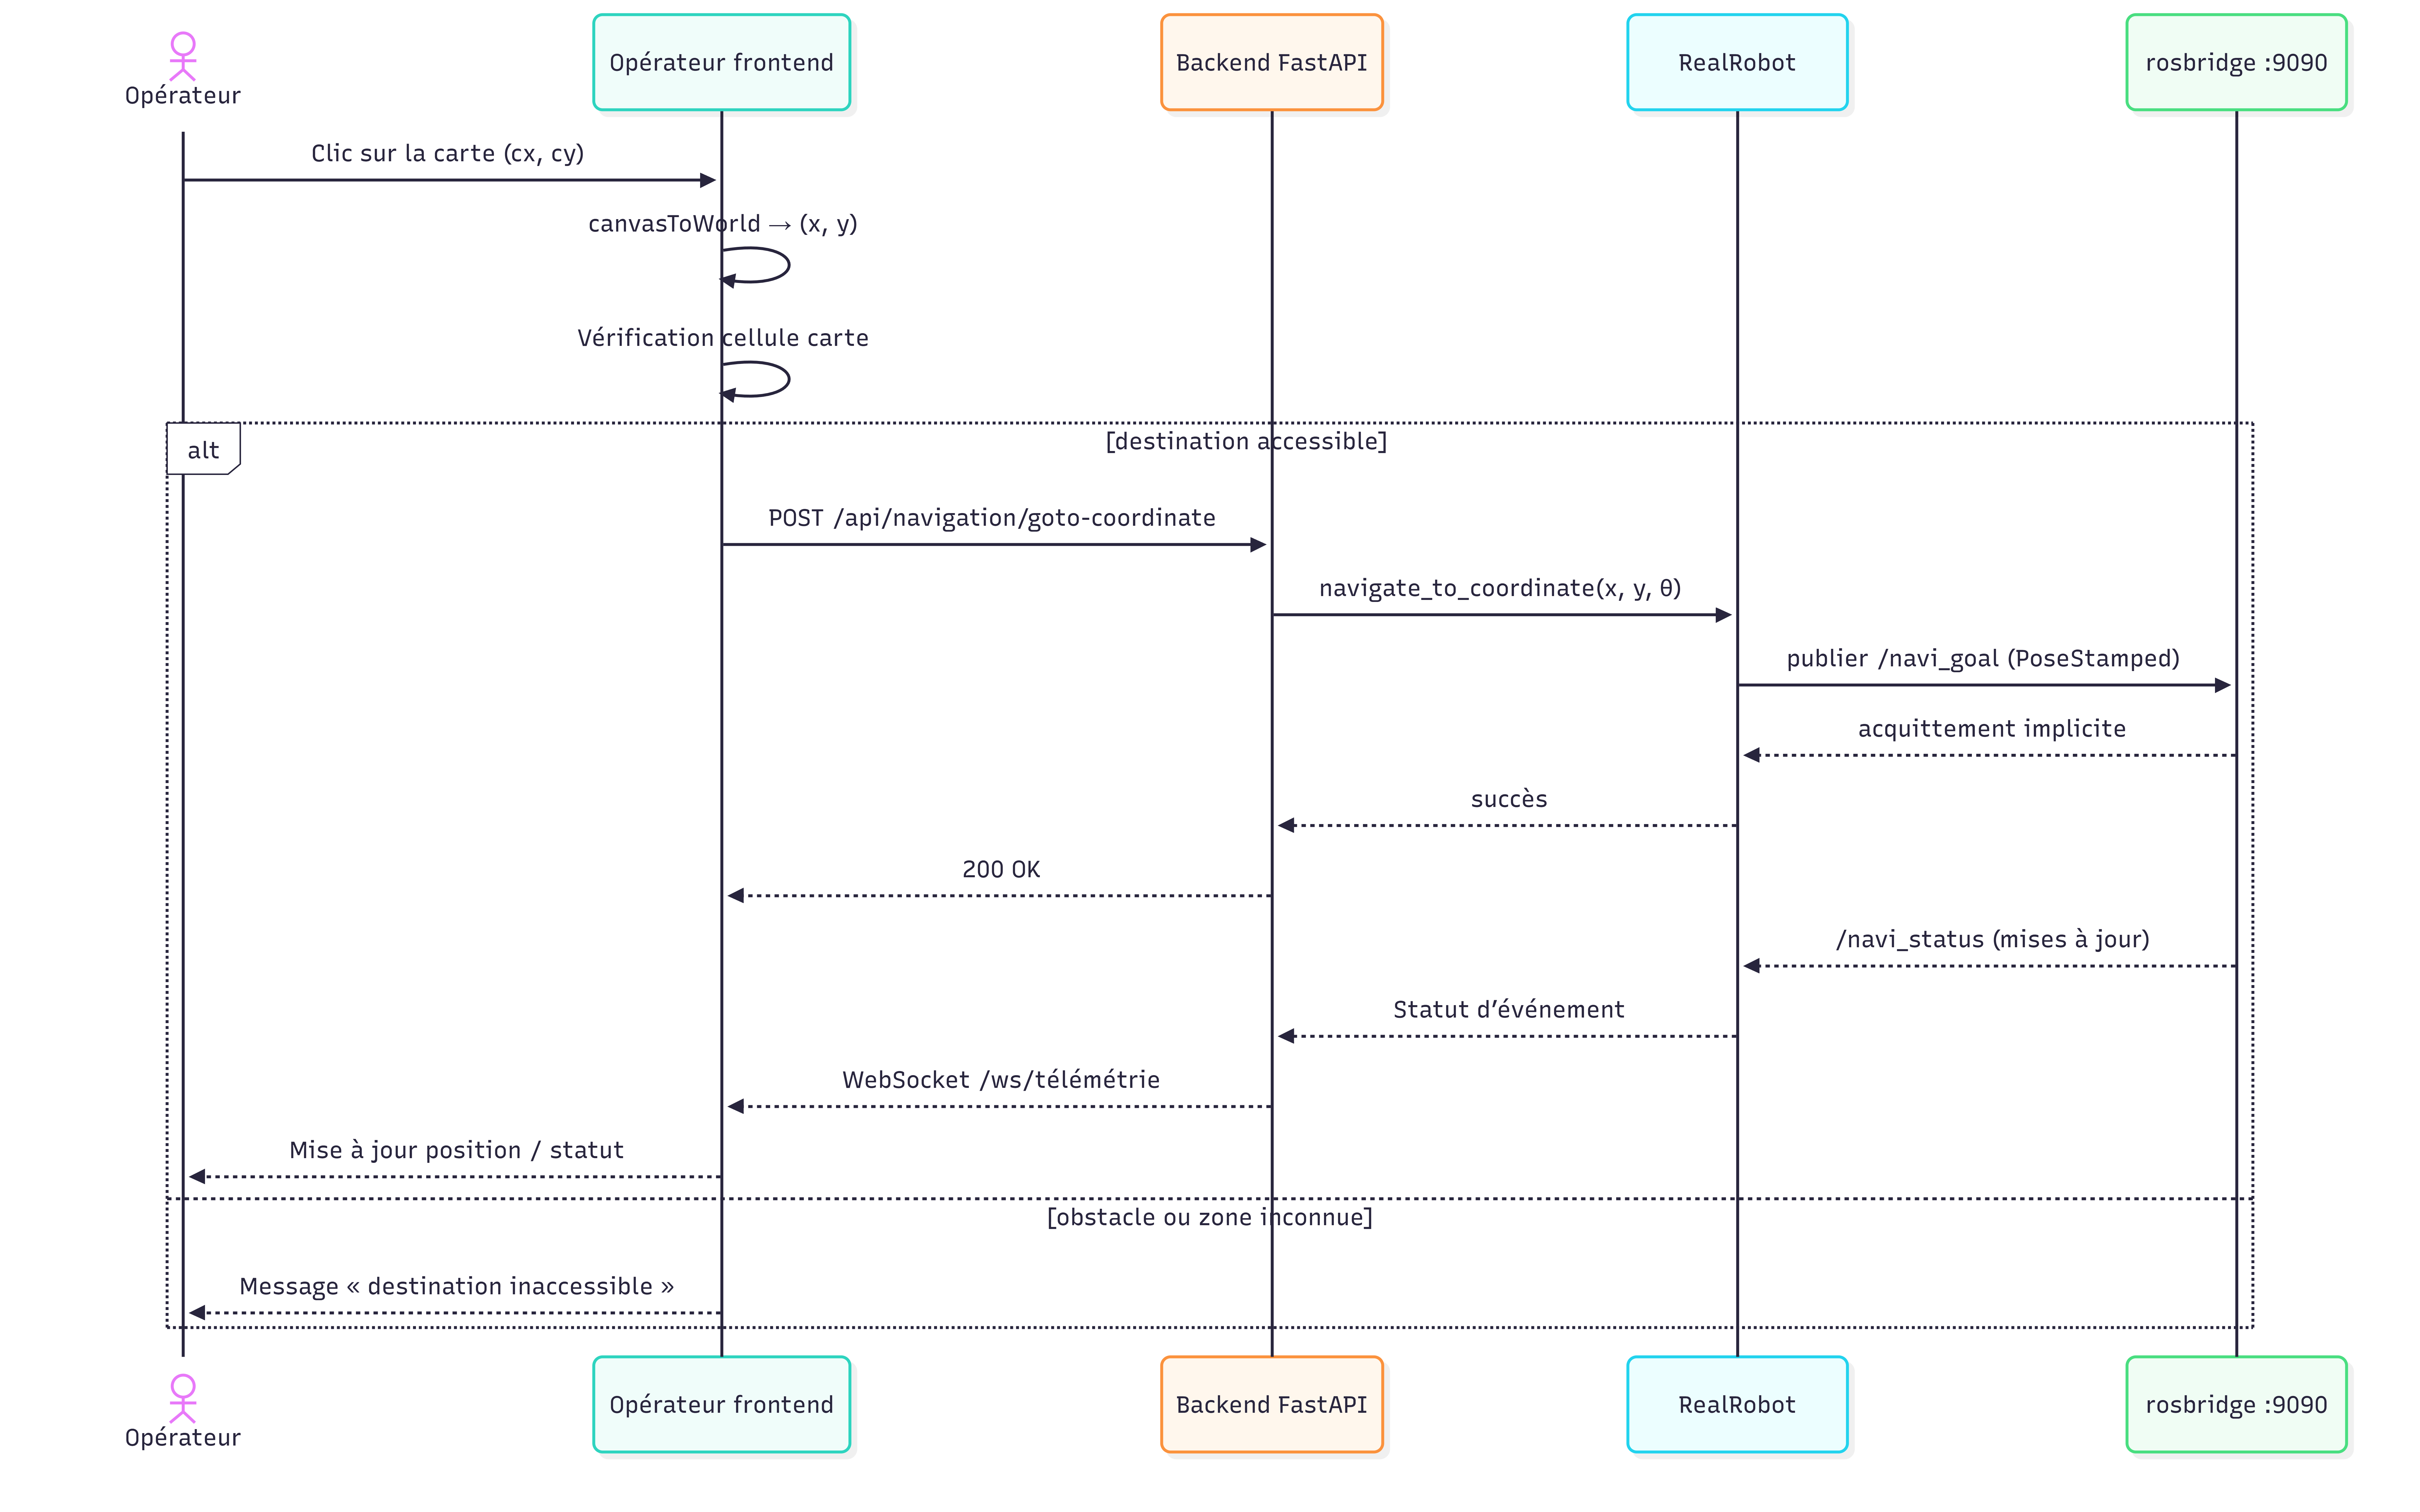
\includegraphics[width=0.85\textwidth]{diagramme/nce_navigation.png-2026-06-20-165623.png}
    \caption{Diagramme de séquence de la navigation vers un point sélectionné}
    \label{fig:diag_sequence}
\end{figure}

\subsection{Modèle des flux de communication}

\subsubsection*{Robot \texorpdfstring{$\leftrightarrow$}{<->} ROSBridge}

ROSBridge constitue la passerelle principale entre la plateforme CYBEL et
le système de navigation du robot. Les échanges reposent sur le protocole
WebSocket et permettent la réception des données de télémétrie,
l'abonnement aux topics ROS, l'appel de services, ainsi que l'envoi de
commandes de navigation et de mouvement.

\subsubsection*{ROSBridge \texorpdfstring{$\leftrightarrow$}{<->} Backend}

Le backend agit comme intermédiaire entre ROSBridge et les interfaces
utilisateur. Il collecte les informations provenant du robot, les traite
puis les redistribue vers les clients connectés. Il assure également la
gestion des commandes envoyées par les utilisateurs.

\subsubsection*{Backend \texorpdfstring{$\leftrightarrow$}{<->} Interfaces utilisateur}

Les interfaces communiquent avec le backend à travers des requêtes REST
pour les actions ponctuelles et des WebSockets pour les mises à jour
temps réel. Cette architecture garantit une supervision réactive et une
faible latence lors de l'affichage des données.

\subsubsection*{Backend \texorpdfstring{$\leftrightarrow$}{<->} Applications Android}

Les applications Android développées dans le cadre du projet permettent
d'étendre les fonctionnalités du système, notamment pour la synthèse
vocale, l'affichage du mode kiosque et les interactions avec la tablette
embarquée.

\subsection{Conclusion}

Ce chapitre a permis de présenter l'analyse fonctionnelle et la conception
générale du système CYBEL. Les besoins identifiés ont conduit à la
définition d'une architecture modulaire organisée autour d'un SDK robot,
d'une API centralisée et de plusieurs interfaces utilisateur. Les
différents diagrammes présentés permettent de visualiser les interactions
entre les acteurs et les composants du système ainsi que les flux de
communication mis en \oe uvre. Cette phase de conception constitue la base
des développements réalisés dans le chapitre suivant, consacré à la
méthodologie et à l'implémentation de la solution proposée.